\documentclass{scrartcl}
\usepackage[utf8]{inputenc}
\usepackage[activate={true,nocompatibility},final,tracking=true,kerning=true,spacing=true,factor=1100,stretch=10,shrink=10]{microtype}
\usepackage[english]{babel}
\usepackage{csquotes}
\usepackage{hyperref}
\usepackage[acronym]{glossaries}
\usepackage[style=ieee, autocite=inline, backend=biber]{biblatex}
\usepackage{siunitx}
\usepackage{todonotes}
\usepackage{parskip}
\usepackage{pgfplots}

\microtypecontext{spacing=nonfrench}
\pgfplotsset{compat=1.15}
\addbibresource{references.bib}

\makenoidxglossaries
\newacronym{api}{API}{Application Programming Interface}
\newacronym{http}{HTTP}{Hyper-Text Transfer Protocol}
\newacronym{json}{JSON}{JavaScript Object Notation}
\newacronym{csv}{CSV}{Comma Seperated Values}

\subject{BUSAN 100G: Digital Information Literacy}
\title{Piazza Visualisation \& Analysis}
\author{Jackson Chadfield}
\date{\today}

\begin{document}

\maketitle

\section{Topic}
I have decided to analyse the annual Stack Overflow developer survey\cite{dataset}.
As a professional programmer, this data is extremely interesting and gives me insight on upcoming technologies to learn.

\section{Source}
Stack Overflow is a knowledge sharing site for programmers and is one of the first places to check when you have a problem related to programming.

Stack Overflow surveys developers using their site annually. It is one of the best sources of data for current trends due to the site being used by so many developers all over the world. Stack Overflow released the anonymous dataset under the Open Database License.

The data is contained in a simple CSV file with 85 columns. The description of what each column is can be found in the schema file published alongside the dataset. In total, the dataset contains \num{88883} rows.

Since the data is for a single year, we cannot calculate trends.

\section{Analysis \& Visualisation}
\subsection{Demographic}
\begin{figure}[p]
    \centering
    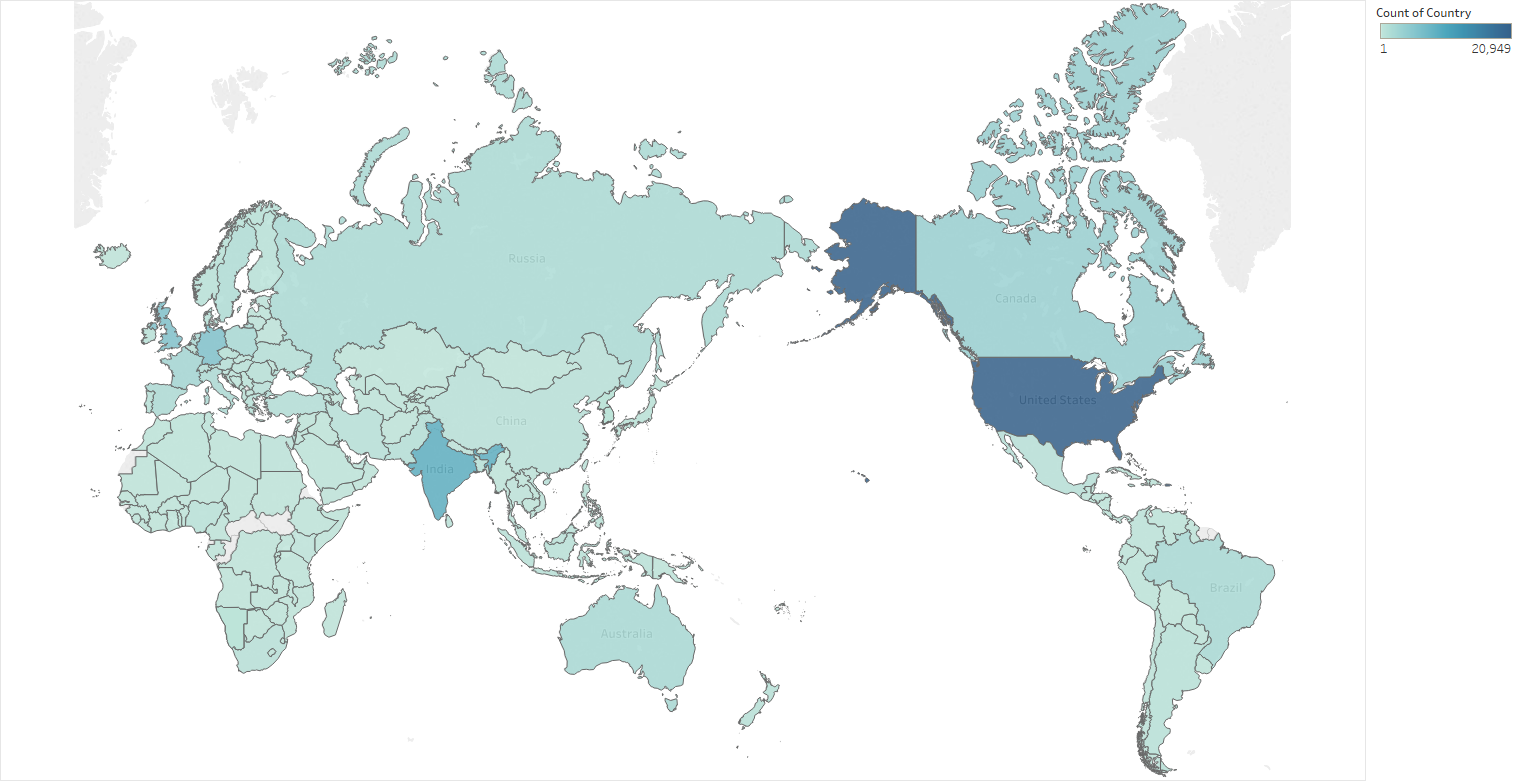
\includegraphics[width=\linewidth]{Documentation/images/map.png}
    \caption{Responses per Country}
    \label{fig:country_responses}
\end{figure}
\begin{figure}[p]
    \centering
    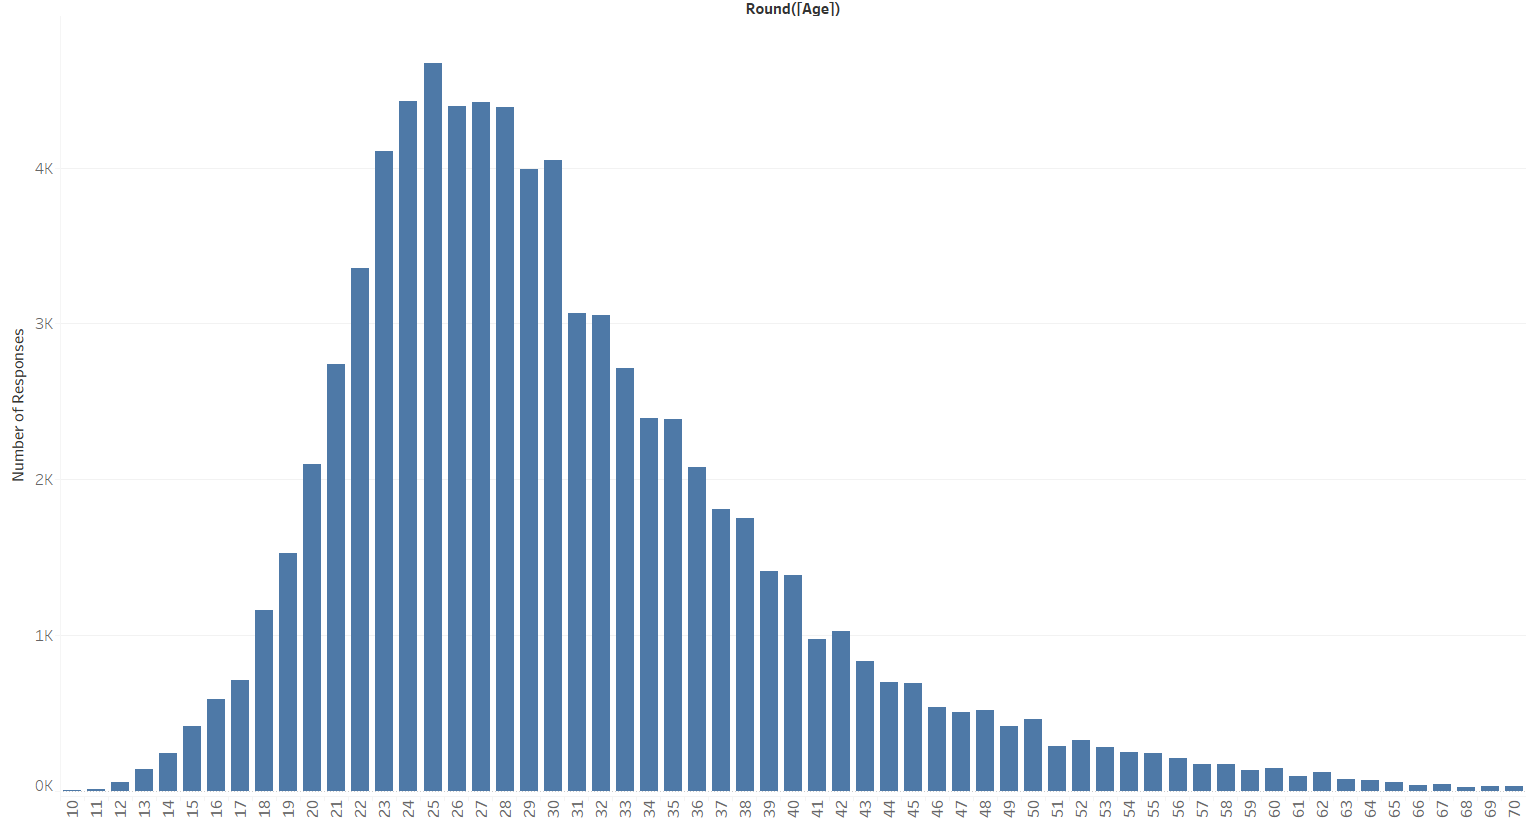
\includegraphics[width=\linewidth]{Documentation/images/age.png}
    \caption{Responses per Age}
    \label{fig:age_responses}
\end{figure}
\begin{figure}[p]
    \centering
    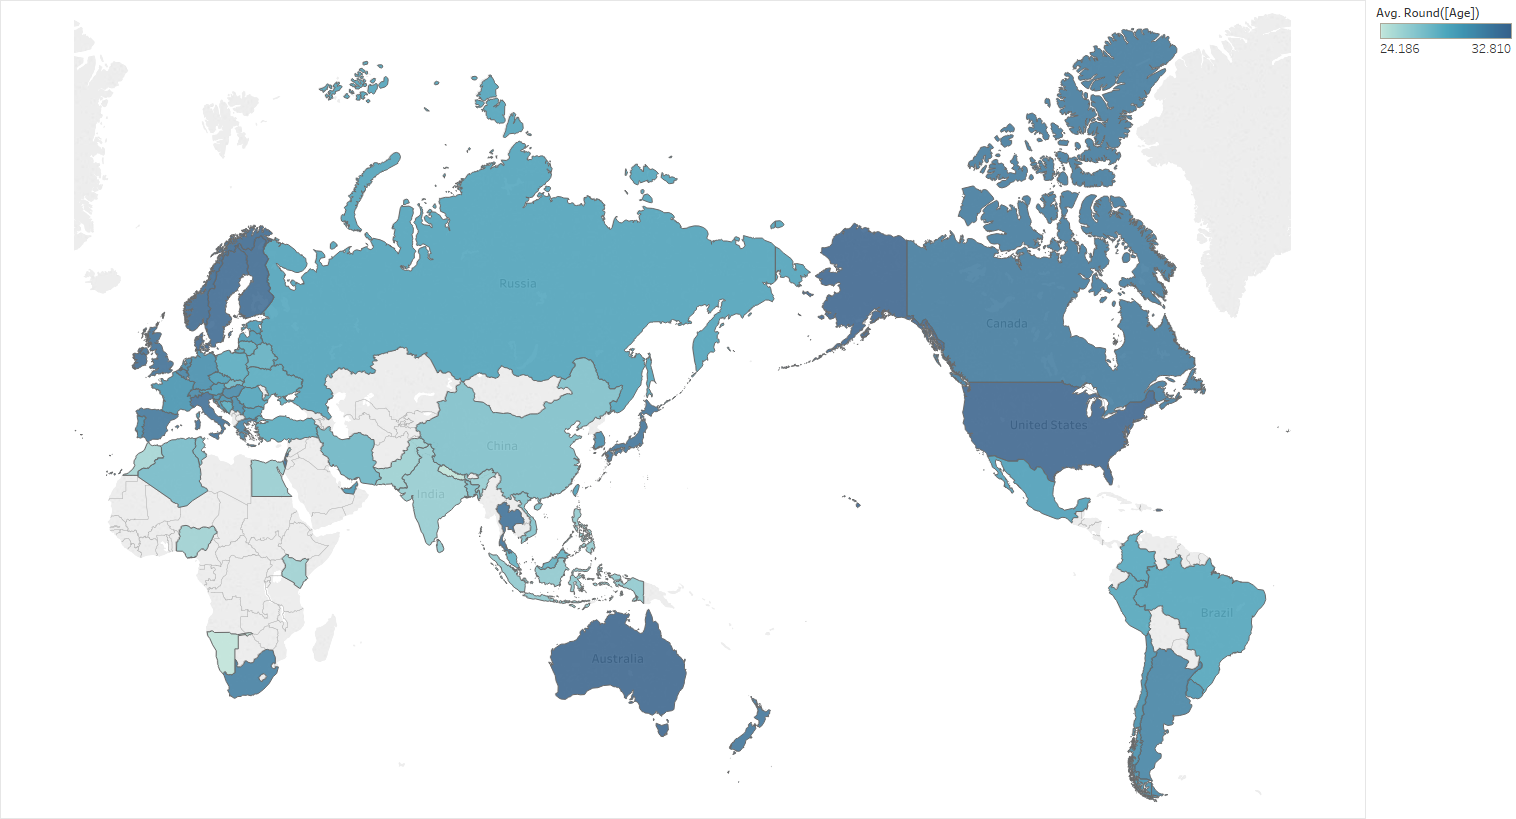
\includegraphics[width=\linewidth]{Documentation/images/average_age.png}
    \caption{Average Age per Country}
    \label{fig:average_age}
\end{figure}
As shown in \autoref{fig:country_responses}, the majority of responses originate from the United States. The second highest country, India has less than half of the United States total responses. Together they form roughly \(\frac{1}{3}\) of the responses. In comparison, New Zealand totals \num{524} responses (~0.6\% of the total responses).

The age of respondents (\autoref{fig:age_responses}) is a normal distribution. With the majority being within \numrange{20}{40} years old. I was also curious about the average age in each country. This can be seen in \autoref{fig:average_age}. I only included countries with 100 or more responses so results wouldn't be skewed by countries with a singular response that is not representative.

\subsection{Academic History}
\begin{figure}[p]
    \centering
    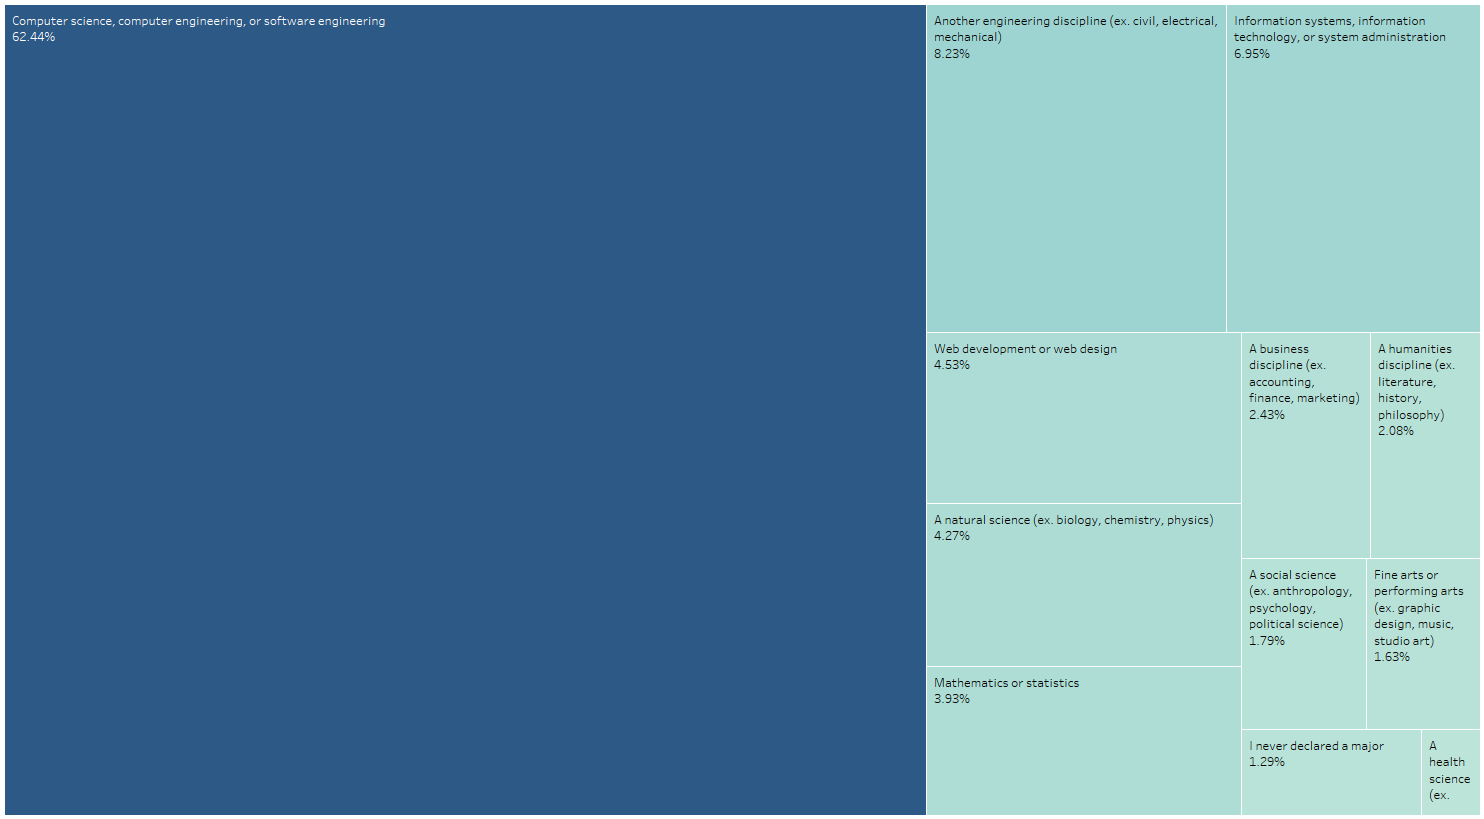
\includegraphics[width=\linewidth]{Documentation/images/majors.png}
    \caption{Majors undertaken by respondents}
    \label{fig:majors}
\end{figure}
As someone currently taking engineering with the intention of specialising in software, I am very interested in the academic paths taken by professional and hobby programmers.

\ref{fig:majors} shows that, unsurprisingly, computer science and software engineering take the top position, with 62.44\%. I am however, surprised that only 1.3\% have not declared a major, as there is a lot of debate online whether it's truly important to have a degree to get a programming job.


\section{Report Management}
This document was written in \LaTeX. Primarily through the online service Overleaf, but also occasionally compiled manually.

I use the distributed version control system git to keep versions of my source code available (this includes both this document and any code used). Since I am the sole contributor to this project and it is relatively small I used a simple linear master branch. I use GitHub as a centralised store for my repository. All versions of my source can be accessed online\footnote{\url{https://github.com/j-chad/piazza-analysis}}

I originally managed my references with Zotero, but found many problems with using it with Bib-\LaTeX{}. The citation keys it generated were messy and many fields were incorrectly populated. I tried Mendeley as an alternative but ultimately found it easier to write the database entries manually.

I use Bib-\LaTeX{} as my back-end for my referencing, which will automatically add a reference list and citations where needed.

This tool-set allows me to access my work from any location: either from overleaf, or by cloning my repository and manually compiling my document.

\printnoidxglossary[type=\acronymtype]
\printbibliography

\end{document}
